\documentclass{article}
\usepackage[utf8]{inputenc}
\usepackage{fancyhdr}
\usepackage[top=1.25in, bottom=1.25in, right=1in, left=1in]{geometry}
\usepackage{graphicx}
\usepackage{amsmath,amsfonts,amssymb,amsthm}
\PassOptionsToPackage{hyphens}{url}\usepackage{hyperref}

\usepackage{etoolbox}
\makeatletter
\patchcmd\g@matrix
 {\vbox\bgroup}
 {\vbox\bgroup\normalbaselines}% restore the standard baselineskip
 {}{}
\makeatother

\pagestyle{fancy}
\fancyhf{}
\rhead{Introduction to Data Science}
\lhead{Predicting Electricity Spot Price}
\rfoot{Page \thepage}
\makeatletter
\renewcommand{\@seccntformat}[1]{}
\makeatother 

%% Theorems etc. %%%%%%%%%%%%%%
%\swapnumbers
\numberwithin{equation}{section}

\makeatletter
\let\c@equation\c@subsection
\makeatother

\title{%
	Predicting Electricity Spot Price\\
	\large Introduction to Data Science Course Project}
\author{Ville Pirsto, Emil Tigerstedt, Ahsan Abbas}

\begin{document}

% Titlepage separately
\begin{titlepage}
	\maketitle
	\thispagestyle{empty}
\end{titlepage}

\tableofcontents
\clearpage

% ---- Introduction ----
\section{Introduction}
This project was done as a part of "Introduction to data science" course in Helsinki University. The focus of this project was to predict the electricity spot prices in Finland for a longer time horizon that is typically available to the consumer. In Finland, the spot electricity prices for the next day are published typically on the previous day after noon, so the spot price horizon is always less than 36 hours. 

Such short price horizon does not allow very long-term planning of electricity consumption. Moreover, there is a psychological effect in play due to uncertainty about the upcoming prices; will I minimize my electricity bill if I do the chores that consume a lot of energy during the price minimum of the current horizon, or will there be even cheaper electricity before I really need to do these chores? One concrete example is charging of ones electric vehicle. Let's say you are planning to drive and see your friends and/or family in the upcoming weekend and it is now monday. You know that you would like to have the battery charged to near-full before your departure on friday afternoon. Should you top up your car battery during the minimum price of the current price horizon, or wait and see if you can save money by postponing until later in the week?

We attempted to address this problem by developing a prediction model for the spot electricity price with longer time horizon. In the spirit of experimentation, we did not got for the most obvious predictor variable there are, such as electricity production from the most dominant sources of energy in Finland (for example, wind and nuclear), or energy exported/imported from other countries. Instead, we attempted to tackle this prediction problem by utilizing more "indirect" predictors.

This report will walk through our project by utilizing the project work canvas. First, the filled canvas is presented, followed by brief discussion on each of the tiles in the canvas.

% ---- Canvas ----
\section{Project Work Canvas}
Figure \ref{fig1} showcases the canvas filled in the beginning of the course (\textbf{Note: Current figure is just the canvas template, to be replaced with our filled canvas}). 


\begin{figure}[htb]
	\centering
	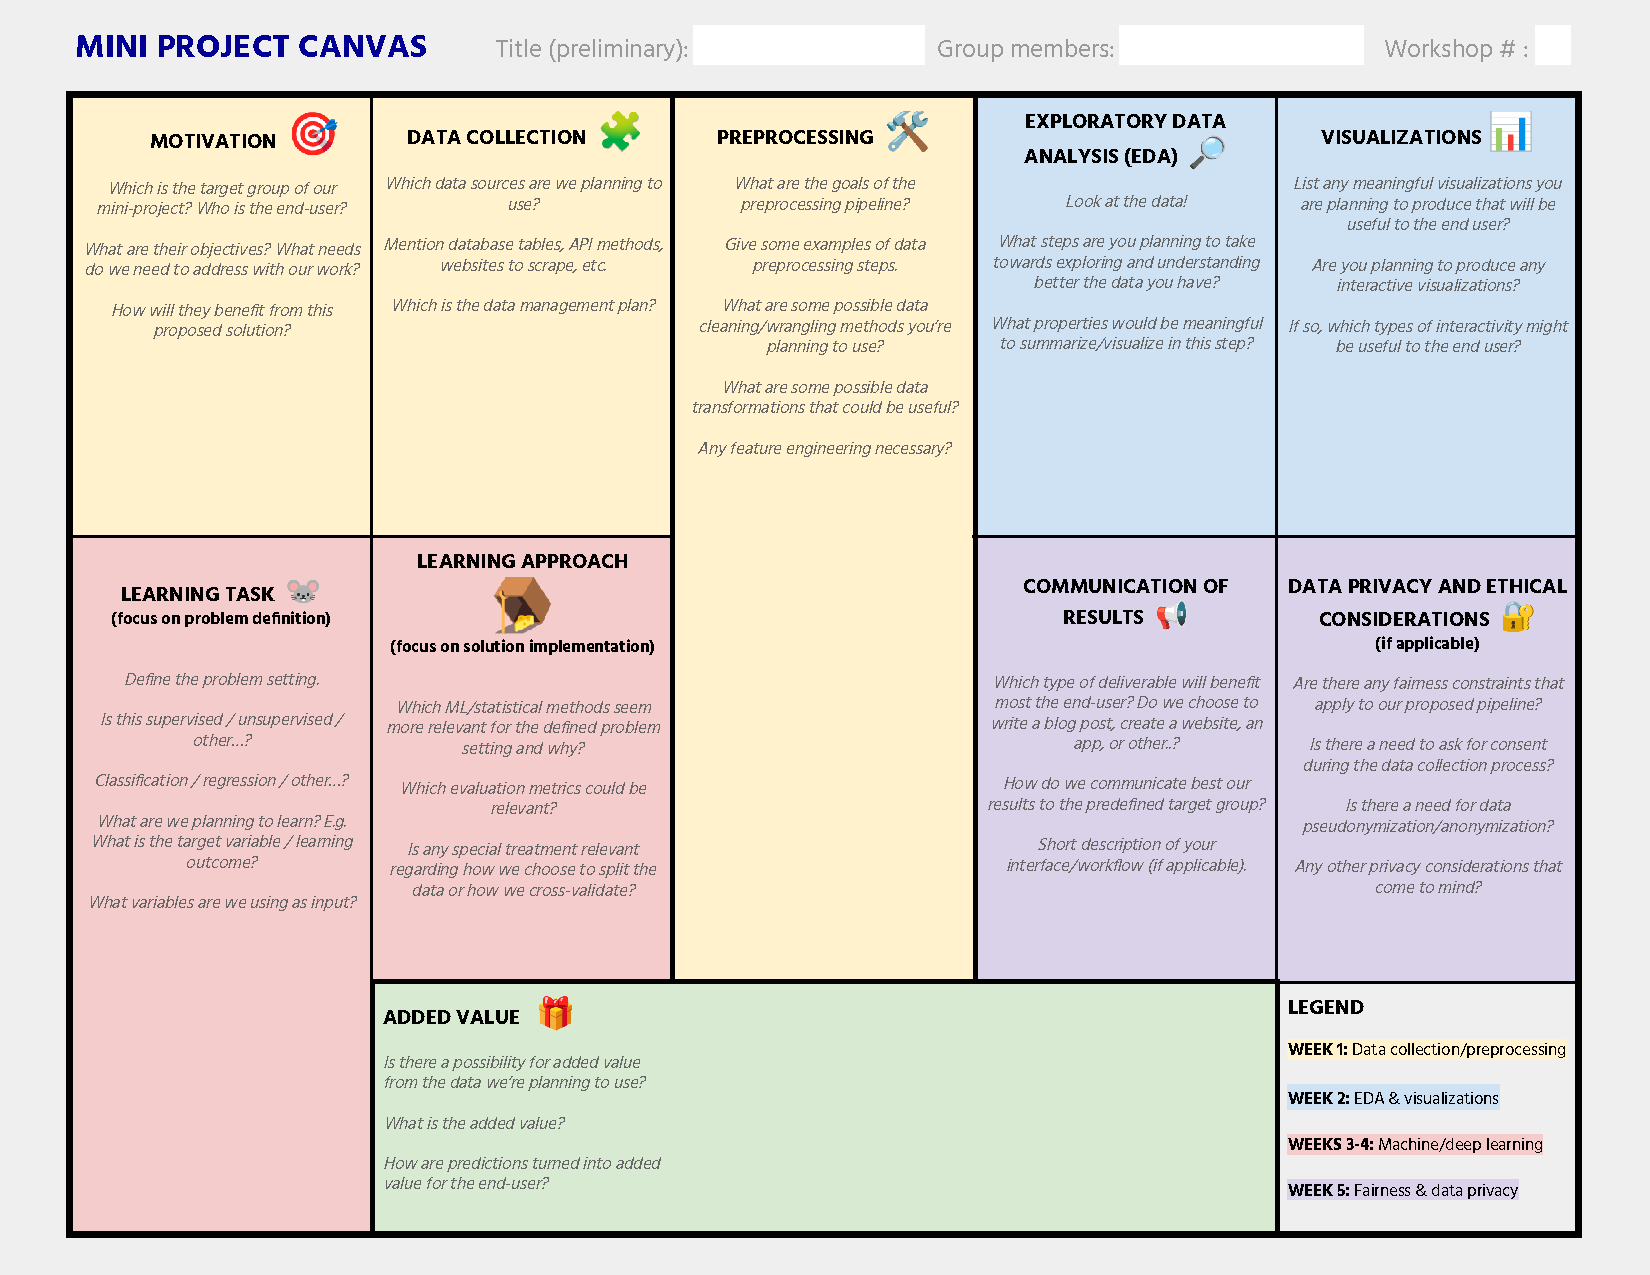
\includegraphics[width=.8\textwidth]{./mini_project_canvas.pdf}
	\caption{Canvas used for project planning.}
	\label{fig1}
\end{figure}

% ---- Data Collection and Preprocessing ----
\section{Data Collection and Preprocessing}
\begin{itemize}
	\item Where is data used from?
	\item How is data stored?
	\item What kind of data is used?
	\item How is data accessed?
	\item What kind of preprocessing is done?

Firstly, we gathered historical spot price data for Finland from \href{https://porssisahko.net/tilastot}{this website}. Additionally, we collected weather data from the \href{https://www.ilmatieteenlaitos.fi/avoin-data/}{Finnish Meteorological Institute} and electricity consumption and production data from Fingrid's open data platform (\href{https://data.fingrid.fi/en/datasets/124}{here} and \href{https://data.fingrid.fi/en/datasets/192}{here}, respectively). All datasets were in Excel format and were downloaded using specific start and end dates as parameters. The data was then imported into a Jupyter notebook using Python, where we created a Pandas DataFrame for each dataset. We then proceeded to preprocess the data to ensure a consistent structure across all datasets.

Preprocessing began with the spot price data, which consisted of two columns: 'Aika' (time) and 'Hinta (snt/kWh)' (price). We adjusted the time column so that prices were aligned with every even hour, and applied this format to the other datasets as well. In the weather data, the year, month, day, and hour were originally in separate columns, so we combined them into a single datetime object. Since the observations were already recorded hourly, no further significant modifications were needed. Different elements of the weather data, such as mean temperature, were stored in separate columns, similar to the structure of the electricity price data.

The electricity consumption and production data, retrieved from the same open data platform, had similar structures. Both datasets included two time-related columns—'startTime' and 'endTime'—along with a column for production or consumption values. We consolidated the two time columns into one, following the same approach used for the weather data. Additionally, the time column still contained extraneous characters, which were cleaned up, and the values were converted into datetime objects.

The main difference between the production and consumption datasets was the frequency of observations: production data was recorded every three minutes, while consumption data was recorded hourly. To standardize the data, we calculated the hourly average for the production data to match the required format.

Once all the datasets were in the correct format, we merged them into a comprehensive dataframe. We then performed imputation, replacing any missing values with the column medians. Finally, we added one more input variable: a boolean variable indicating whether the date of an observation fell on a public holiday. The public holiday dates were sourced from \href{https://www.officeholidays.com/countries/finland/2021}{this website} .

All the data collection and preprocessing described above was carried out in a single Jupyter notebook. In addition, we created three separate Jupyter notebooks, each dedicated to handling one API. These APIs were used to fetch weather, electricity consumption, and electricity production forecasts for the upcoming days. The API used for the weather forecast is available in \href{https://api.open-meteo.com/v1/forecast}{here}, and the data retrieved required no significant preprocessing. Electricity consumption and production predictions were collected via APIs available on the same Fingrid open data platform as the historical data. Since the prediction data had a structure very similar to the historical data, we were able to reuse the preprocessing methods to bring the predictions into the desired format.
\end{itemize}

% ---- EDA and Visualizations ----
\section{Exploratory Data Analysis and Visualizations}
\begin{itemize}
	\item What kind of EDA was done?
	\item How was the data visualized?
	\item What kind of findings were obtained?
\end{itemize}
We began the exploratory data analysis by creating pair plots using functions from the Seaborn library, which generated scatter plots and kernel density estimate plots for each variable pair. To enhance the interpretability of these plots, we added a hue to distinguish data points as either 'day' or 'night.' This was done by introducing a new column, time_of_day, with values of 'day' or 'night' based on the hour of each observation: observations from 6:00 to 18:00 were labeled as day, and those from 18:00 to 6:00 as night. The pair plots did not reveal any notable patterns, with one clear exception: electricity consumption was generally lower at night than during the day.

% ---- Learning ----
\section{Learning to Predict Electricity Spot prices}
During the project, we focused on three different approaches to predict the electricity spot price. Our initial plan was to apply time series modeling to fit a model that would capture both the seasonality of the prices both day- and year-wise. Seasonality was captured quite well by to model, but it was not able to capture the significant day-to-day variations that occur in the spot prices due to various reasons. One major contributing factor here was probably the choice of predictors, but we wanted to keep the number of inputs low. Nevertheless, after considerable effort in tuning and trying different time series models, we had to concede on this front.

Our second approach was to use XGBoost machine learning algorithm to do the predictions. \textbf{some explanations here on it...}

Finally, we utilized the TPOT library introduced in the exercises of the course to suggest us a model. TPOT proposed to apply random forest algorithm, and so we did. As predicted by TPOT, it turned out to yield the best prediction accuracy out of the models we had tried so far.

\begin{itemize}
	\item What kind of approaches were tried?
	\item What kind of observations were made during this process?
	\item What approach was used in the end? Why? How did we end up to it?
\end{itemize}

% ---- Communciation of Results ----
\section{Communication of Results}
\begin{itemize}
	\item Webpage, how?
	\item What kind of user interface is used?
	\item What does the webpage do? What can the user do?
\end{itemize}

% ---- Summary ----
\section{Summary}
As it turns out, predicting electricity spot prices is difficult. The machinery behind the price fluctuations is complex and can not be explained through weather and directly related predictors. Indeed, one needs to consider not only national, but international weather and electricity markets. Moreover, thorough coverage of the various significant electricity production forms in Finland should be included in the mix. Considering the future continuation of this project, one might try to add more predictors that are directly tied to the electricity market. 

Nevertheless, the participants considered the project successful. Each one learned something new along the way. Some highlights of the themes we learned about include data preprocessing and formatting for learning, familiarizing ourselves with different artificial intelligence models, learning to use APIs for data collection, getting comfortable with version control, and planning short business pitches. Last, but not the least, we also improved our collaboration and communication skills.



% ----------------------------------------------------------------
\iffalse
\begin{figure}[htb]
\centering
\includegraphics[width=.5\textwidth]{./largestEigenvalue.eps}
\caption{Suurimman ominaisarvon approksimaatiovirheen itseisarvo $i$:n funktiona.}
\label{fig1}
\end{figure}
\fi

\end{document}
